\documentclass[aps,prl,twocolumn,superscriptaddress,floatfix]{revtex4-2}

\usepackage{amsmath,amssymb}
\usepackage{graphicx}
\usepackage{hyperref}
\usepackage{xcolor}

\begin{document}

\title{The Geometry of Learning: Data Complexity Controls the Fractal Dimension of Gradient Descent}

\author{Evan Paul}
\email{evan@example.com}
\affiliation{Independent Researcher}

\date{\today}

\begin{abstract}
We measure the fractal dimension of neural network training trajectories in function space. Using the Grassberger-Procaccia correlation dimension $D_2$, we find that a convolutional network trained on CIFAR-10 with full-batch gradient descent produces a strange attractor with $D_2 = 3.67 \pm 0.08$ at 30\% of the Edge of Stability threshold. Persistent homology confirms fractal rather than smooth manifold topology. Cross-architecture controls reveal that data complexity is the necessary ingredient for multi-dimensional chaos, while architecture modulates the learning-rate threshold at which it appears: a multilayer perceptron on the same data reaches $D_2 = 4.35 \pm 0.06$ near the Edge of Stability, whereas either architecture on structureless synthetic data remains at $D_2 \approx 0.9$. Lyapunov exponents peak at intermediate learning rates and become negative at high learning rates as basin convergence dominates. Peak chaos and peak geometric complexity dissociate---the attractor is most complex in the transition zone between chaotic and basin-convergent regimes. These results provide a geometric characterization of training dynamics consistent with the Newhouse-Ruelle-Takens route to chaos.
\end{abstract}

\maketitle

\section{Introduction}

Gradient descent is a deterministic dynamical system. Each update maps the network's function to a new function, producing a trajectory through function space whose geometry can be measured.

Recent work has established that this geometry is nontrivial. Cohen \textit{et al.}~\cite{cohen2021} discovered the Edge of Stability (EoS): the top Hessian eigenvalue rises to $2/\eta$ and oscillates rather than diverging. Damian \textit{et al.}~\cite{damian2023} characterized the self-stabilization mechanism. Kalra \textit{et al.}~\cite{kalra2025} and Ghosh \textit{et al.}~\cite{ghosh2025} observed period-doubling near the EoS, and Morales \textit{et al.}~\cite{morales2024} computed Lyapunov exponents during training, establishing that the dynamics can be chaotic. Storm \textit{et al.}~\cite{storm2024} showed that finite-time Lyapunov exponents through network depth form coherent structures in input space.

These results establish that training dynamics are rich, but leave open a geometric question: what \textit{shape} does the chaos have? A chaotic trajectory might be essentially one-dimensional---erratic motion along a single convergence path---or it might fill a multi-dimensional fractal volume. We measure this distinction using the correlation dimension $D_2$~\cite{grassberger1983} and find that training trajectories settle onto strange attractors whose fractal dimension is controlled by data complexity and modulated by architecture.

\section{Experimental Framework}

\textit{Architectures and data.}---We study five conditions under full-batch gradient descent with MSE loss, no momentum, and no weight decay (Table~\ref{tab:conditions}). Full-batch training isolates the deterministic dynamics. Learning rates are expressed as fractions of $2/\lambda_{\max}$, where $\lambda_{\max}$ is the top Hessian eigenvalue after 1{,}000 warmup steps at $\eta = 0.01$. All networks are trained for 5{,}000 steps.

The CNN has two convolutional layers ($3{\to}16{\to}32$ channels, $3{\times}3$ kernels, max pooling, ReLU, two fully connected layers; 268{,}650 parameters) trained on a 2{,}000-image CIFAR-10 subset. The MLPs use 2-hidden-layer tanh networks of width 50 (156K parameters) or 85 (269K parameters) on either CIFAR-10 (flattened) or synthetic data (220 dimensions, 10 classes). The CNN-on-synthetic condition embeds synthetic data into $3{\times}32{\times}32$ tensors to isolate architectural effects.

\textit{Lyapunov exponents.}---We measure chaos in function space to avoid overparameterization artifacts. Two copies of the network train from identical initialization, one perturbed by $\varepsilon = 10^{-5}$ along a random unit-norm direction. The function-space divergence $\delta(t) = \lVert f(\mathbf{x}) - \tilde{f}(\mathbf{x}) \rVert$ is recorded on 100 held-out inputs; $\lambda$ is the slope of $\ln\delta(t)$ versus $t$ over $[0.2T, 0.8T]$. Sensitivity analysis confirms that $\varepsilon = 10^{-8}$ produces uniform artifactual positive exponents; $\varepsilon \geq 10^{-6}$ is required for converged measurements~\cite{sm}. Results are averaged over 10 seeds (CNN/CIFAR-10), 3 seeds (cross-experiments), or 20 seeds (MLP/synthetic).

\textit{Correlation dimension.}---$D_2$ is computed via the Grassberger-Procaccia algorithm~\cite{grassberger1983} on function-space trajectories (outputs recorded every 10 steps, first 20\% discarded as transient, yielding ${\sim}400$ points). Pipeline validation recovers $D_2 = 2.06$ for a quasiperiodic 2-torus (expected 2.0) and $D_2 = 1.68$ for the Lorenz attractor (expected 2.05). Extended calibration~\cite{sm} reveals a systematic 15--35\% underestimate for fractal attractors; reported values are conservative lower bounds.

\begin{figure*}[t]
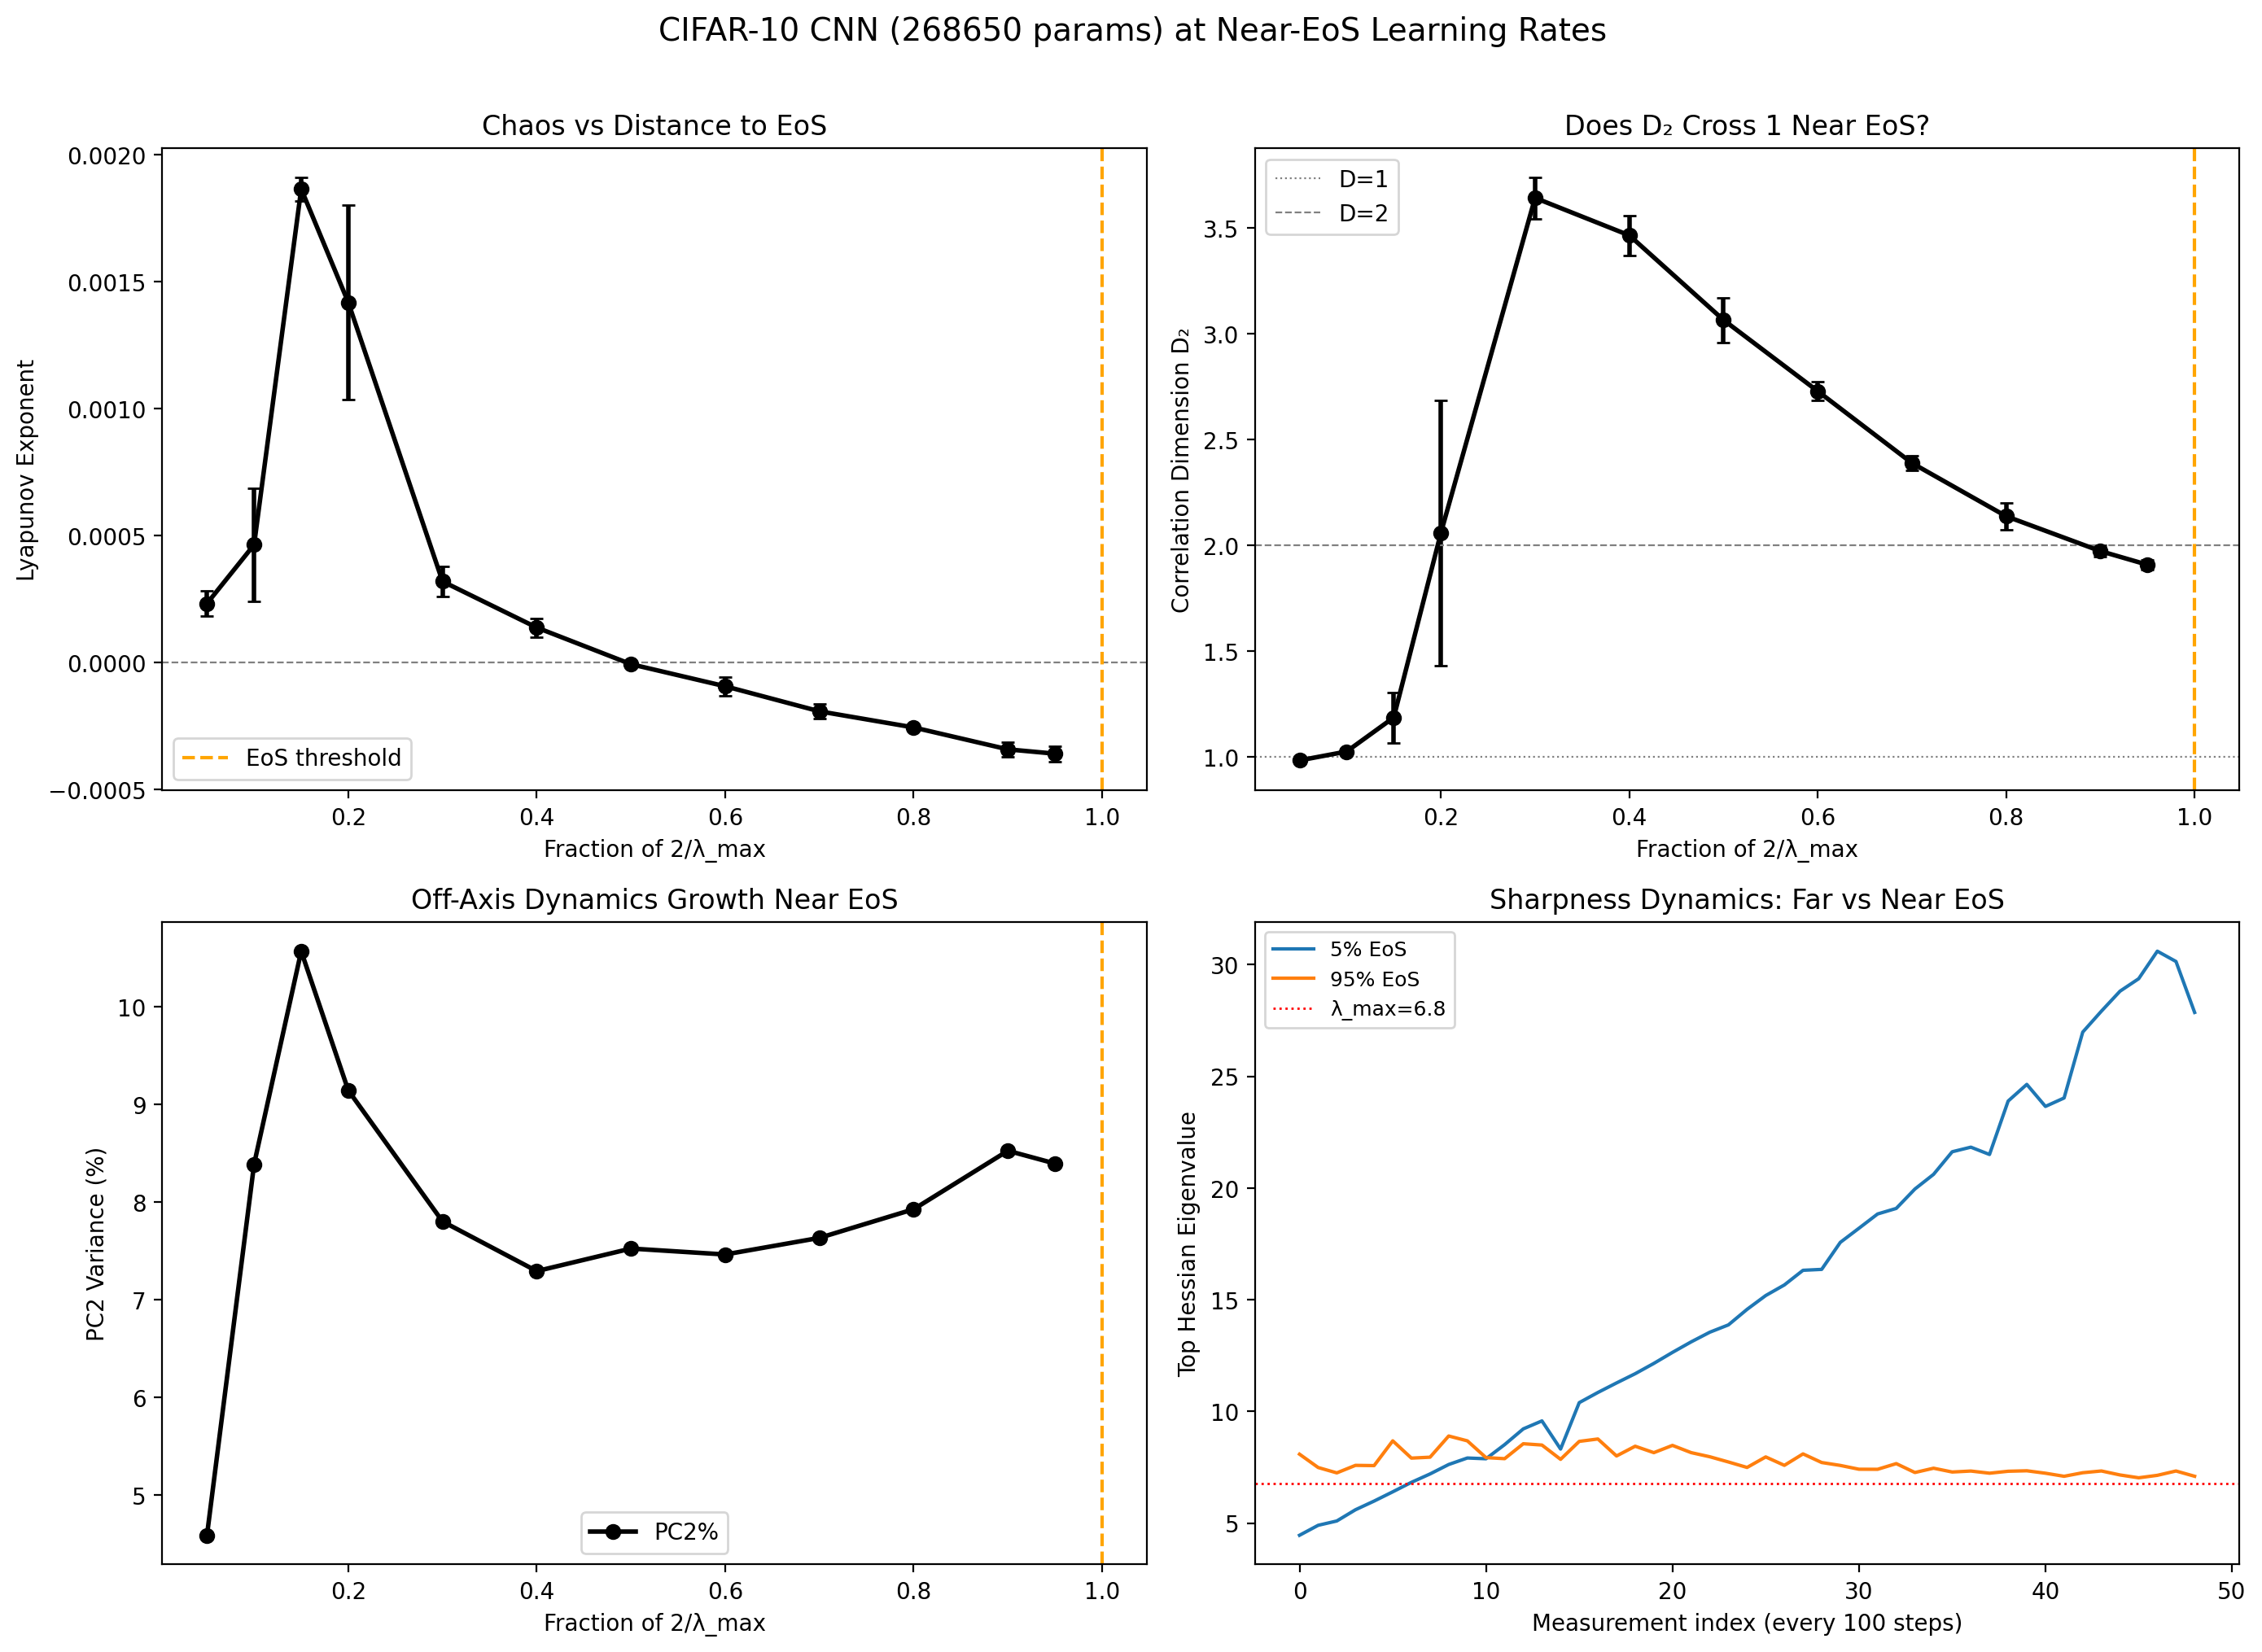
\includegraphics[width=\textwidth]{cifar10_eos.png}
\caption{\label{fig:cnn}%
CNN (268{,}650 parameters) on CIFAR-10, 10 seeds.
(a)~Lyapunov exponent versus fraction of the EoS threshold $2/\lambda_{\max}$. The chaos window peaks at 15\% and closes near 45\%.
(b)~Correlation dimension $D_2$. The trajectory crosses $D_2 = 1$ at 10\% of EoS and peaks at $3.67 \pm 0.08$ at 30\%.
(c)~Second principal component variance, showing off-axis dynamics.
(d)~Sharpness time series: monotonic progressive sharpening at 5\% EoS (blue) versus bounded oscillation at 95\% EoS (orange). Error bars: standard deviation across seeds.}
\end{figure*}

\textit{Persistent homology.}---Computed via \textsc{ripser}~\cite{ripser} on PCA-reduced trajectories to distinguish smooth tori (few persistent loops, large gap ratio) from strange attractors (many features at all scales, gap ratio ${\approx}1$).

\section{Results}

\textit{The chaos window.}---The Lyapunov exponent is non-monotonic with learning rate [Fig.~\ref{fig:cnn}(a)]. In the CNN on CIFAR-10, $\lambda$ peaks at 15\% of the EoS threshold and crosses zero near 45\%. Above this, basin convergence dominates: trajectories from different perturbations collapse to the same learned function. This bounded chaos window appears in every architecture tested; its width scales with architecture complexity.

\textit{Training trajectories are strange attractors.}---Within the chaos window, the CNN/CIFAR-10 trajectory acquires fractal structure [Fig.~\ref{fig:cnn}(b)]. $D_2$ crosses 1.0 at 10\% of EoS, rises through $2.63 \pm 0.62$ at 20\%, peaks at $3.67 \pm 0.08$ at 30\%, and remains above 2.0 to 80\% of EoS. The first principal component captures only ${\sim}52$\% of trajectory variance---half the dynamics are off the primary convergence axis. Since our pipeline underestimates fractal dimensions by 15--35\%, the true attractor dimension is likely substantially higher.

Persistent homology confirms fractal topology. At 30\% of EoS, 386 $H_1$ features appear with gap ratio 1.2 (no dominant loops); at 40\%, 421 $H_1$ and 401 $H_2$ features. At 5\% of EoS, zero $H_1$ features: a simple convergence path. This is the topological signature of a strange attractor---many holes at all scales---not a smooth torus.

\textit{Data complexity is the engine; architecture is the throttle.}---The cross-architecture controls (Table~\ref{tab:conditions}, Fig.~\ref{fig:cross}) reveal a clean hierarchy. A CNN on structureless synthetic data produces $D_2 < 1.0$ at all learning rates---architecture alone is insufficient. A parameter-matched MLP (269K) on CIFAR-10 reaches $D_2 = 4.35 \pm 0.06$ at 90\% of EoS; a smaller MLP (156K) reaches $D_2 = 4.56 \pm 0.02$. Data complexity is both necessary (CNN + synthetic $\to$ $D_2 \approx 1$) and sufficient (MLP + CIFAR-10 $\to$ $D_2 > 4$).

Architecture modulates the \textit{threshold}: at 30\% of EoS the CNN has already reached $D_2 = 3.67$ while both MLPs remain at $D_2 \approx 1$. The MLPs require 70--90\% of EoS to achieve comparable fractal dimension. The convolutional hierarchy facilitates mode coupling at lower learning rates.

\textit{Peak chaos and peak complexity dissociate.}---Peak $\lambda$ occurs at 15\% of EoS; peak $D_2$ at 30\%. The attractor is geometrically most complex not where perturbation sensitivity is greatest, but in the transition zone where chaotic dynamics and basin convergence compete. This dissociation is characteristic of the KAM transition regime~\cite{kam}, where ordered and chaotic regions coexist in fractal interleaving.

\begin{table}[b]
\caption{\label{tab:conditions}%
Experimental conditions with $D_2$ at each condition's peak.}
\begin{ruledtabular}
\begin{tabular}{lccccc}
 & Params & Data & Peak $D_2$ & EoS\% & $N$\\
\hline
MLP/synth. & 14K & synth. & 0.9 & all & 20\\
CNN/synth. & 269K & synth. & ${\sim}1.0$ & all & 3\\
MLP/CIFAR & 156K & C-10 & $4.56(2)$ & 90 & 3\\
MLP/CIFAR & 269K & C-10 & $4.35(6)$ & 90 & 3\\
CNN/CIFAR & 269K & C-10 & $3.67(8)$ & 30 & 10\\
\end{tabular}
\end{ruledtabular}
\end{table}

\begin{figure}[t]
\includegraphics[width=\columnwidth]{figure2_cross_experiments_v2.png}
\caption{\label{fig:cross}%
$D_2$ versus fraction of the EoS threshold for all five conditions. CNN on CIFAR-10 (red circles, 10 seeds) peaks at 30\% EoS; MLPs on CIFAR-10 (blue squares, green triangles, 3 seeds) peak at 90\% EoS. Synthetic conditions (open markers) remain at $D_2 \approx 1$ throughout. Error bars: standard deviation across seeds.}
\end{figure}

\section{Discussion}

These results provide a geometric characterization of gradient descent: the trajectory through function space is a strange attractor whose fractal dimension depends on what the network is learning and how it is structured.

The findings are consistent with the Newhouse-Ruelle-Takens route to chaos~\cite{ruelle1971,newhouse1978}. Complex data creates a loss landscape with ridges, saddle points, and near-equivalent solutions that provide independent axes of oscillation. When enough of these modes couple through the training dynamics, the flow produces a strange attractor. The bounded chaos window is consistent with the KAM picture~\cite{kam}: some invariant structures survive perturbation while others are destroyed, and peak geometric complexity appears in the transition zone. The CNN's hierarchical processing creates efficient coupling pathways, lowering the learning rate at which the transition occurs. The MLP accesses the same modes---provided by the data---but requires stronger driving to couple them. On structureless data, no architecture produces multi-dimensional dynamics because the modes do not exist.

These dynamical findings complement Pittorino \textit{et al.}~\cite{pittorino2022}, who showed that the loss landscape has toroidal topology after symmetry removal---a static geometric property of the parameter space on which these dynamical transitions unfold.

A methodological note: Lyapunov exponents computed at perturbation scale $\varepsilon = 10^{-8}$ are dominated by numerical noise~\cite{sm}. Reliable measurements require $\varepsilon \geq 10^{-6}$. Prior work at smaller $\varepsilon$~\cite{morales2024} should be interpreted with caution. The function-space protocol avoids false positives from gauge symmetries in overparameterized networks.

Several questions remain open. Does the attractor structure persist under stochastic gradient descent? Does $D_2$ continue to grow with larger architectures and datasets? Networks trained within the chaos window are known to generalize better~\cite{cohen2021}, and our measurements show these are the learning rates that produce strange attractors. Whether this connection is causal---whether exploring a higher-dimensional attractor during training produces better solutions---is the central question these measurements now enable.

\begin{acknowledgments}
Portions of this manuscript were drafted with the assistance of AI language models (Claude, Anthropic). All experimental design, data collection, analysis, and scientific interpretation were performed by the authors. Source code, raw data, and analysis scripts are available at \url{https://github.com/gnomevan/attractor}.
\end{acknowledgments}

\bibliography{references}

\end{document}
